\documentclass[conference]{IEEEtran}
\IEEEoverridecommandlockouts

\usepackage{cite}
\usepackage{amsmath,amssymb,amsfonts}
\usepackage{algorithmic}
\usepackage{graphicx}
\usepackage{textcomp}
\usepackage{xcolor}
\usepackage{siunitx}
\usepackage[brazil]{babel}
\usepackage[utf8]{inputenc}
\usepackage{float} % <-- Adicionado para controlar posição das figuras

\def\BibTeX{{\rm B\kern-.05em{\sc i\kern-.025em b}\kern-.08em
    T\kern-.1667em\lower.7ex\hbox{E}\kern-.125emX}}
\begin{document}

\title{Utilizando algoritmos de aprendizagem de máquina em um braço robótico simulado }

\author{\IEEEauthorblockN{Lucca Santos Cerasomma}
\IEEEauthorblockA{\textit{Graduação em Engenharia da Computação} \\
\textit{FHO - Uniararas}\\
Araras, Brasil \\
luccacerasomma@alunos.fho.edu.br}
}

\maketitle

\section{Introdução}
A manipulação de objetos é uma das principais  tarefas da robótica. É muito comum que os movimentos dos braços robóticos sejam calculados por trajetória e análise de valores lidos por sensores para realização de um movimento mais preciso. Embora os métodos clássicos sejam eficiente, esse pesquisa vai abordar o uso de algoritmos de aprendizagem por reforço para que o ao invés de programar cada movimento do braço robótico o ele mesmo irá aprender como se comportar e concluir tarefas, com o tentativas e erros e uma política de maximização como um sinal de recompensa.
Para a construção do modelo, o trabalho vai ter como proposta o uso de renderização em OpenGl, em que um braço simulado deve aprender a pegar caixas. Mas como aspecto de confiabilidade nos movimentos, o algoritmo será treinado para também respeitar angulações, para ter um movimento semelhante ao braço humano.
O ambiente o OpenGl é essencial para o funcionamento e andamento do projeto, já que o uso algoritmo de aprendizagem por reforço (AR) em robôs reais seria financeiramente inviável os modelos de computação gráfica permitem a visualização e testes com algoritmos rodando localmente.

\section{Metodologia}
No aprendizado por reforço (RL), o agente interage com o ambiente em passos de tempo discretos. A cada instante, ele observa um estado $s_t$, seleciona uma ação $a_t$ e recebe uma recompensa $r_t$ (positiva ou negativa), transitando em seguida para um novo estado $s_{t+1}$. Diferente do aprendizado supervisionado, o agente deve aprender a partir das consequências de suas próprias ações, balanceando os processos de exploração (\textit{exploration}) e aproveitamento (\textit{exploitation}), com o objetivo de maximizar o retorno acumulado (SCHULMAN et al., 2017).

Para este trabalho, empregam-se e comparam-se dois algoritmos: o \textit{Proximal Policy Optimization} (PPO), descrito a seguir, e o \textit{Soft Actor-Critic} (SAC), descrito na Seção~\ref{sec:sac}. Os métodos de gradiente de política, como o PPO, parametrizam uma política estocástica $\pi_\theta(a_t \mid s_t)$ e estimam o gradiente do objetivo a partir de trajetórias amostradas por meio de:

\begin{equation}
    \hat{g} = \hat{\mathbb{E}}_t \left[ \nabla_\theta \log \pi_\theta(a_t \mid s_t) \hat{A}_t \right]
    \label{eq:policy_gradient}
\end{equation}

\noindent onde $\hat{A}_t$ denota o estimador da função de vantagem no instante $t$.

Embora como primeira ideia seria reutilizar a mesma trajetória em múltiplos passos de otimização, essa abordagem carece de garantia teórica e, empiricamente, provoca passos de atualização destrutivamente grandes na política (SCHULMAN et al., 2017). Para contornar essa instabilidade, o PPO define a razão de probabilidades entre a política atual e a anterior:

\begin{equation}
    r_t(\theta) = \frac{\pi_\theta(a_t \mid s_t)}{\pi_{\theta_{\text{old}}}(a_t \mid s_t)}
    \label{eq:ratio}
\end{equation}

\noindent e otimiza uma função objetivo truncada (\textit{clipped surrogate objective}):

\begin{equation}
    \begin{aligned}
        L^{\text{CLIP}}(\theta) = \hat{\mathbb{E}}_t \Big[ \min \big( & r_t(\theta)\hat{A}_t, \\
        & \text{clip}(r_t(\theta), 1-\epsilon, 1+\epsilon)\hat{A}_t \big) \Big]
    \end{aligned}
    \label{eq:ppo_clip}
\end{equation}

\noindent onde $\epsilon$ é um hiperparâmetro (tipicamente $\epsilon = 0{,}2$). O operador de corte restringe a variação da razão de probabilidades ao intervalo $[1-\epsilon, 1+\epsilon]$. Com isso, ações associadas a vantagens positivas têm sua probabilidade elevada e ações com vantagens negativas têm sua probabilidade reduzida, porém sem permitir que atualizações com valores errados desequilibrem o desempenho da política.

\subsection{Ambiente de simulação}

O ambiente foi implementado em Python seguindo a interface da biblioteca Gymnasium, na qual o agente interage com a simulação por meio de duas operações: o reinício de um episódio e a execução de um passo, que recebe uma ação e devolve o novo estado, a recompensa e a indicação de término. A simulação (cinemática do braço, preensão e recompensa) foi separada da renderização, feita com OpenGL.

O braço é composto por três segmentos rígidos, de comprimentos $L_1 = 0{,}50$~m, $L_2 = 0{,}40$~m e $L_3 = 0{,}20$~m, ligados por três juntas rotacionais (ombro, cotovelo e punho), montados sobre um pedestal de altura $h_b = 0{,}10$~m, com uma garra de dois dedos na extremidade. Todas as juntas giram em torno do mesmo eixo ($z$), de modo que o movimento ocorre em um plano vertical. Cada junta possui limites angulares que impedem a rotação completa, conforme a Tabela~\ref{tab:juntas}.

\begin{table}[htb]
    \centering
    \caption{Limites angulares das juntas}
    \label{tab:juntas}
    \begin{tabular}{lccc}
        \hline
        Junta & Comprimento (m) & $\theta_{\min}$ & $\theta_{\max}$ \\
        \hline
        Ombro    & 0,50 & $10^\circ$   & $170^\circ$ \\
        Cotovelo & 0,40 & $-150^\circ$ & $150^\circ$ \\
        Punho    & 0,20 & $-120^\circ$ & $120^\circ$ \\
        \hline
    \end{tabular}
\end{table}

O ângulo do ombro é medido em relação ao chão e os demais em relação ao segmento anterior. Sendo $\phi_i = \sum_{k=1}^{i} \theta_k$ o ângulo acumulado até a junta $i$, a posição da extremidade $\mathbf{p} = (x, y)$ é obtida por cinemática direta:

\begin{equation}
    \begin{aligned}
        x &= \sum_{i=1}^{3} L_i \cos \phi_i \\
        y &= h_b + \sum_{i=1}^{3} L_i \sin \phi_i
    \end{aligned}
    \label{eq:cinematica}
\end{equation}

O objeto é uma caixa cúbica de $0{,}08$~m de aresta, posicionada no chão no início de cada episódio com a coordenada $x$ sorteada uniformemente no intervalo $[0{,}35;\,0{,}85]$~m, dentro do alcance do braço. Adotou-se um modelo de preensão simplificado, sem simulação de atrito: a caixa é considerada presa quando a abertura da garra é menor que $0{,}3$ e a distância entre a extremidade e o centro da caixa é menor que $0{,}05$~m. Enquanto presa, a caixa acompanha a extremidade; se a abertura ultrapassar $0{,}5$, a caixa é solta e cai $0{,}02$~m por passo até o chão.

Na renderização, cada segmento é um cubo unitário escalado e cada junta é uma esfera. O braço é desenhado por modelagem hierárquica com a pilha de matrizes do OpenGL: para cada junta, aplica-se uma rotação pelo ângulo $\theta_i$ em torno do eixo $z$, desenha-se o segmento e aplica-se uma translação de comprimento $L_i$ até a junta seguinte, de modo que a transformação de cada segmento acumula as de todos os anteriores. A cena usa projeção em perspectiva, iluminação com uma fonte pontual e teste de profundidade (\textit{Z-buffer}). O resultado da renderização é mostrado na Figura~\ref{fig:braco}.

\begin{figure}[htb]
    \centering
    \includegraphics[width=\columnwidth]{Imagem,_braco_robo.png}
    \caption{Braço robótico, caixa e cenário renderizados em OpenGL. A linha verde indica a altura-alvo da tarefa.}
    \label{fig:braco}
\end{figure}

\subsection{Formulação do problema}

\subsubsection{Espaço de estados}

O estado $s_t$ fornecido à política é um vetor de 17 valores reais:

\begin{equation}
    s_t = \big[\, \sin\boldsymbol{\theta},\, \cos\boldsymbol{\theta},\, \tilde{\boldsymbol{\theta}},\, g,\, \mathbf{p},\, \mathbf{c},\, \mathbf{c} - \mathbf{p},\, b \,\big]
    \label{eq:estado}
\end{equation}

\noindent em que $\boldsymbol{\theta} \in \mathbb{R}^3$ são os ângulos das juntas, $\tilde{\boldsymbol{\theta}}$ são esses ângulos normalizados para $[-1, 1]$ em relação aos seus limites, $g \in [0, 1]$ é a abertura da garra, $\mathbf{p}$ e $\mathbf{c}$ são as posições $(x, y)$ da extremidade e do centro da caixa, e $b \in \{0, 1\}$ indica se a caixa está presa. A representação dos ângulos por seno e cosseno evita descontinuidades, e o vetor $\mathbf{c} - \mathbf{p}$ informa diretamente a direção até o objeto. A política recebe esses valores numéricos, e não a imagem renderizada.

\subsubsection{Espaço de ações contínuo}

A ação é um vetor contínuo $a_t \in [-1, 1]^4$. As três primeiras componentes definem a variação angular das juntas e a quarta, a variação da abertura da garra:

\begin{equation}
    \begin{aligned}
        \theta_i &\leftarrow \text{clip}\big(\theta_i + a_{t,i}\,\Delta\theta_{\max},\; \theta_{\min,i},\; \theta_{\max,i}\big) \\
        g &\leftarrow \text{clip}\big(g + a_{t,4}\,\Delta g_{\max},\; 0,\; 1\big)
    \end{aligned}
    \label{eq:acao}
\end{equation}

\noindent com $\Delta\theta_{\max} = 4^\circ$ e $\Delta g_{\max} = 0{,}2$ por passo. A saturação da Equação~\eqref{eq:acao} implementa os limites mecânicos da Tabela~\ref{tab:juntas}. No PPO, a política $\pi_\theta(a_t \mid s_t)$ é uma distribuição normal multivariada diagonal, cuja média é produzida pela rede do ator e cujo desvio-padrão é um parâmetro treinável independente do estado. Durante o treinamento, as ações são amostradas dessa distribuição, o que garante a exploração; na avaliação, utiliza-se apenas a média.

\subsubsection{Função de recompensa}

Utilizou-se uma recompensa moldada em etapas:

\begin{equation}
    \begin{aligned}
        r_t ={}& \begin{cases}
            -1 - d_t, & \text{caixa não presa} \\
            -(h^{*} - h_t), & \text{caixa presa}
        \end{cases} \\
        & + 2\,\mathbf{1}_{\text{pega}} + 10\,\mathbf{1}_{\text{sucesso}} \\
        & - 0{,}01\,\lVert a_t \rVert^2 - 0{,}5\,\mathbf{1}_{\text{chão}}
    \end{aligned}
    \label{eq:recompensa}
\end{equation}

\noindent em que $d_t = \lVert \mathbf{c} - \mathbf{p} \rVert$ é a distância entre a extremidade e a caixa, $h_t$ é a altura da caixa em relação ao chão, $h^{*} = 0{,}40$~m é a altura-alvo, $\mathbf{1}_{\text{pega}}$ vale 1 apenas na primeira vez em que a caixa é agarrada no episódio, $\mathbf{1}_{\text{sucesso}}$ vale 1 quando a caixa presa atinge $h^{*}$ e $\mathbf{1}_{\text{chão}}$ vale 1 quando alguma junta fica abaixo do chão. Como a recompensa por passo é negativa até o sucesso, o agente é incentivado a concluir a tarefa rapidamente. Além disso, qualquer estado com a caixa presa (recompensa entre $-0{,}4$ e $0$) é melhor que qualquer estado sem ela (no máximo $-1$), o que torna a preensão sempre vantajosa. O bônus de preensão é concedido uma única vez, para evitar que o agente aprenda a pegar e soltar a caixa repetidamente.

\subsubsection{Episódios}

Cada episódio começa com o braço na postura $(90^\circ, -60^\circ, -60^\circ)$, a garra aberta e a caixa em posição sorteada. O episódio termina com sucesso quando a caixa presa atinge a altura $h^{*}$, ou é interrompido (truncado) após 250 passos.

\subsection{Procedimento de treinamento do PPO}

O treinamento segue um ciclo repetido até atingir o total de passos definido:

\begin{enumerate}
    \item \textbf{Coleta:} oito cópias independentes do ambiente, cada uma com uma posição de caixa sorteada, são executadas em paralelo com a política atual $\pi_{\theta_{\text{old}}}$ por 1.024 passos, totalizando 8.192 transições. Para cada uma, são armazenados o estado, a ação, a recompensa e a probabilidade da ação sob a política atual;
    \item \textbf{Vantagem:} o crítico estima o valor $V_\phi(s_t)$ dos estados coletados e as vantagens $\hat{A}_t$ são calculadas pelo método \textit{Generalized Advantage Estimation} (SCHULMAN et al., 2015), com $\gamma = 0{,}99$ e $\lambda = 0{,}95$;
    \item \textbf{Otimização:} por 10 épocas, as transições são embaralhadas e divididas em 32 minilotes de 256 amostras; o ator é atualizado pela Equação~\eqref{eq:ppo_clip}, com a razão $r_t(\theta)$ da Equação~\eqref{eq:ratio} limitada ao intervalo $[0{,}8;\,1{,}2]$, e o crítico, pelo erro quadrático entre o valor estimado e o retorno observado;
    \item \textbf{Descarte:} as transições são descartadas, pois deixam de representar a política atualizada, e um novo ciclo de coleta é iniciado.
\end{enumerate}

A cada 10.000 passos, o agente é avaliado em 20 episódios em um ambiente separado, usando a ação média (política determinística), e são registrados o retorno médio e a taxa de sucesso. O modelo com maior retorno médio nessas avaliações é salvo. Neste trabalho foi utilizada uma semente aleatória (semente 0). Na máquina utilizada, o PPO processou aproximadamente 2.000 passos por segundo, sem renderização. Ao final, o melhor modelo é avaliado em 100 episódios, com posições de caixa definidas pelas sementes 1000 a 1099, e visualizado em OpenGL.

\subsection{Soft Actor-Critic (SAC)}
\label{sec:sac}

Como segundo algoritmo, foi utilizado o \textit{Soft Actor-Critic} (SAC) (HAARNOJA et al., 2018a), que difere do PPO em dois aspectos. O primeiro é ser \textit{off-policy}: em vez de descartar as transições após cada atualização, o SAC as armazena em uma memória de repetição (\textit{replay buffer}) $\mathcal{D}$ e as reutiliza muitas vezes, inclusive aquelas geradas por versões anteriores da política. O segundo é seguir o princípio de máxima entropia: além do retorno, o agente maximiza a entropia da política, o que o incentiva a manter comportamentos variados enquanto isso não comprometer a recompensa:

\begin{equation}
    J(\pi) = \sum_{t} \mathbb{E}_{\rho_\pi} \Big[ r(s_t, a_t) + \alpha \, \mathcal{H}\big(\pi(\cdot \mid s_t)\big) \Big]
    \label{eq:sac_objetivo}
\end{equation}

\noindent em que $\rho_\pi$ é a distribuição de pares $(s_t, a_t)$ visitados pela política, $\mathcal{H}(\pi(\cdot \mid s_t)) = -\mathbb{E}_{a \sim \pi}[\log \pi(a \mid s_t)]$ é a entropia da política e $\alpha > 0$ é a temperatura, que regula o peso da exploração em relação à recompensa.

O SAC utiliza um ator $\pi_\theta$ e dois críticos $Q_{\phi_1}$ e $Q_{\phi_2}$, que estimam o valor de um par estado-ação, além de cópias desses críticos, as redes-alvo $Q_{\bar{\phi}_1}$ e $Q_{\bar{\phi}_2}$, que se atualizam lentamente. Os críticos são treinados com a equação de Bellman na versão ``suave'', que inclui o termo de entropia no valor do estado seguinte:

\begin{equation}
    \begin{aligned}
        y = r + \gamma (1 - d) \Big( & \min_{j=1,2} Q_{\bar{\phi}_j}(s', \tilde{a}') \\
        & - \alpha \log \pi_\theta(\tilde{a}' \mid s') \Big)
    \end{aligned}
    \label{eq:sac_alvo}
\end{equation}

\begin{equation}
    L_Q(\phi_j) = \mathbb{E}_{\mathcal{D}} \left[ \big( Q_{\phi_j}(s, a) - y \big)^2 \right]
    \label{eq:sac_critico}
\end{equation}

\noindent em que $\tilde{a}' \sim \pi_\theta(\cdot \mid s')$ é uma ação amostrada da política atual no estado seguinte, $d$ indica o término do episódio, $j = 1, 2$, e as transições $(s, a, r, s', d)$ são sorteadas de $\mathcal{D}$. O uso do menor valor entre os dois críticos reduz a tendência de superestimação dos valores, comum em métodos ator-crítico (FUJIMOTO et al., 2018).

A política é uma distribuição normal cuja média $\mu_\theta(s)$ e desvio-padrão $\sigma_\theta(s)$ são produzidos pela rede do ator, seguida de uma tangente hiperbólica que mantém as ações no intervalo $[-1, 1]$. Para que o gradiente do crítico possa ser propagado até o ator, a ação é escrita como função determinística dos parâmetros e de um ruído independente $\xi \sim \mathcal{N}(0, I)$ (truque de reparametrização):

\begin{equation}
    \tilde{a}_\theta(s, \xi) = \tanh\big( \mu_\theta(s) + \sigma_\theta(s) \odot \xi \big)
    \label{eq:sac_reparam}
\end{equation}

\noindent e o ator é atualizado para escolher ações de alto valor e alta entropia, minimizando:

\begin{equation}
    \begin{aligned}
        L_\pi(\theta) = \mathbb{E}_{s, \xi} \Big[ & \alpha \log \pi_\theta\big(\tilde{a}_\theta(s, \xi) \mid s\big) \\
        & - \min_{j=1,2} Q_{\phi_j}\big(s, \tilde{a}_\theta(s, \xi)\big) \Big]
    \end{aligned}
    \label{eq:sac_ator}
\end{equation}

A temperatura $\alpha$ é ajustada automaticamente (HAARNOJA et al., 2018b), de modo a manter a entropia da política próxima de um valor-alvo $\bar{\mathcal{H}}$:

\begin{equation}
    L(\alpha) = \mathbb{E}_{a \sim \pi_\theta} \left[ -\alpha \big( \log \pi_\theta(a \mid s) + \bar{\mathcal{H}} \big) \right]
    \label{eq:sac_alpha}
\end{equation}

\noindent Por fim, as redes-alvo seguem os críticos por média móvel exponencial, $\bar{\phi}_j \leftarrow \tau \phi_j + (1 - \tau) \bar{\phi}_j$, o que estabiliza o alvo da Equação~\eqref{eq:sac_alvo}.

\section{Resultados}

Os resultados a seguir correspondem a uma execução de cada configuração (semente 0). Durante o treinamento, os agentes foram avaliados a cada 10.000 passos em 20 episódios com a política determinística. Ao final, o melhor modelo de cada configuração foi avaliado em 100 episódios, com as posições da caixa definidas pelas sementes 1000 a 1099, as mesmas para todos os agentes.

\subsection{Curvas de aprendizado}

A Figura~\ref{fig:curvas} apresenta a evolução do retorno médio e da taxa de sucesso ao longo do treinamento. As curvas começam em 10.000 passos, que é o momento da primeira avaliação; por isso, o primeiro ponto já reflete o que cada agente aprendeu nesse intervalo, e não o comportamento sem treino.

% figure* = figura ocupando as duas colunas (no IEEEtran ela vai para o topo da página)
\begin{figure*}[t]
    \centering
    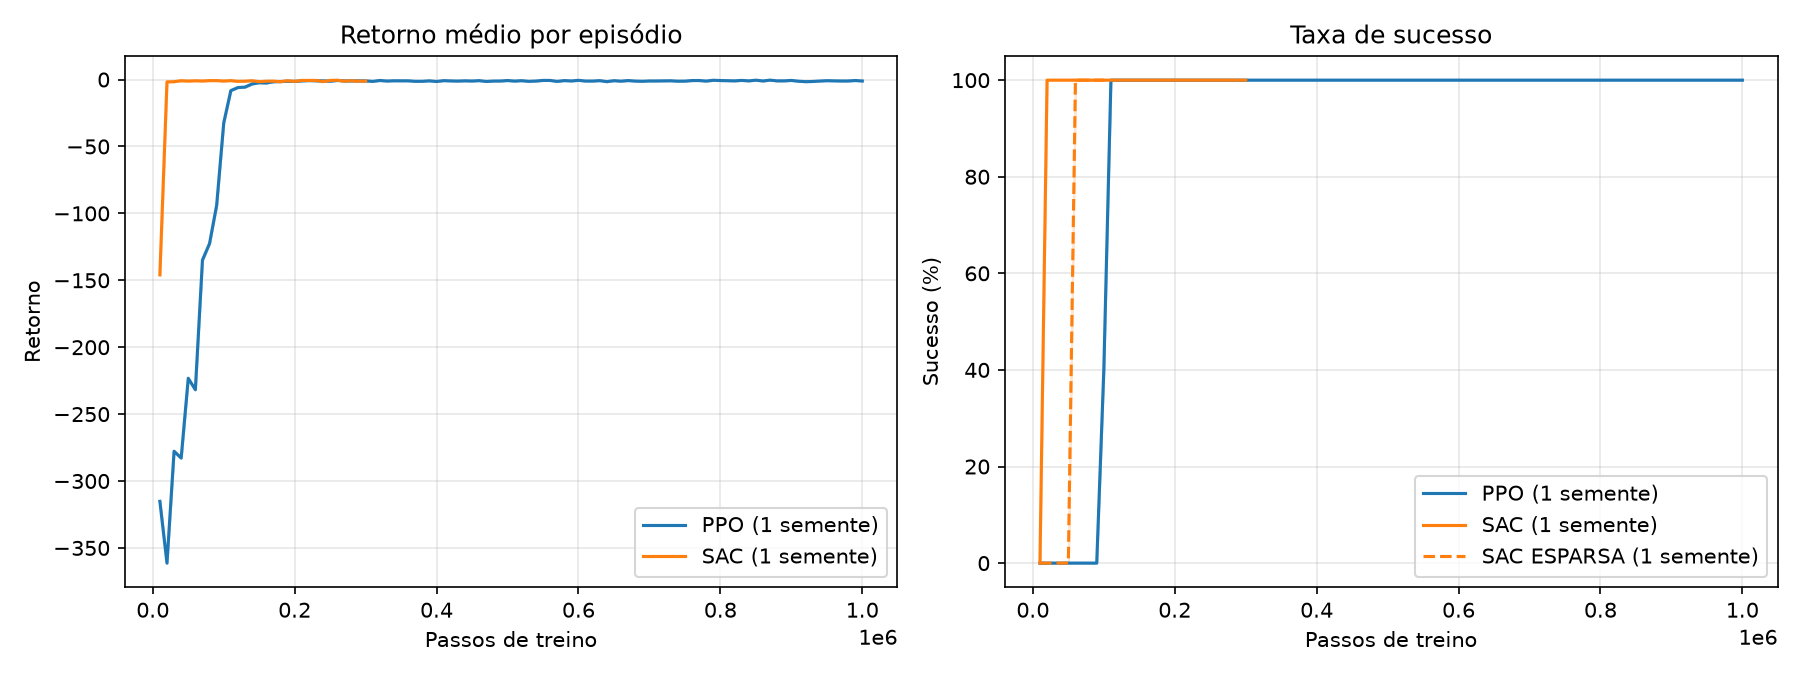
\includegraphics[width=\textwidth]{resultados.png}
    \caption{Retorno médio por episódio (esquerda) e taxa de sucesso (direita) em função dos passos de treinamento. A linha tracejada corresponde ao SAC treinado com recompensa esparsa, mostrado apenas na taxa de sucesso por ter retorno em outra escala.}
    \label{fig:curvas}
\end{figure*}

No SAC, o retorno médio passou de $-145{,}9$ na avaliação de 10.000 passos para $-1{,}7$ na de 20.000 passos, quando a taxa de sucesso atingiu 100\%, e permaneceu nesse patamar até o fim dos 300.000 passos. O valor de $-145{,}9$ indica que, com 10.000 passos, dos quais os 5.000 primeiros foram de ações aleatórias, o agente já agarrava a caixa em parte dos episódios, embora ainda não a elevasse até a altura-alvo: como cada passo sem a caixa custa pelo menos $-1$ e os episódios sem sucesso duram 250 passos, um agente que nunca agarrasse a caixa teria retorno inferior a $-250$.

No PPO, a evolução foi mais gradual. O retorno partiu de $-315{,}2$ com 10.000 passos, oscilou entre $-360$ e $-220$ até 60.000 passos e subiu de forma consistente a partir daí, chegando a $-32{,}4$ com 100.000 passos, quando a taxa de sucesso foi de 40\%. A partir de 110.000 passos, a taxa de sucesso chegou a 100\% e se manteve até o fim do treinamento, com 1.000.000 de passos, e o retorno se estabilizou em torno de $-1$.

\subsection{Eficiência de amostras}

A Tabela~\ref{tab:eficiencia} resume a quantidade de passos de treinamento necessária para que cada agente atingisse 100\% de sucesso nas avaliações periódicas. Como as avaliações ocorrem a cada 10.000 passos, os valores indicam o primeiro ponto avaliado em que isso ocorreu.

\begin{table}[htb]
    \centering
    \caption{Passos de treinamento até 100\% de sucesso nas avaliações}
    \label{tab:eficiencia}
    \begin{tabular}{lcc}
        \hline
        Configuração & Último 0\% & Primeiro 100\% \\
        \hline
        SAC (etapas)   & 10.000 & 20.000 \\
        PPO (etapas)   & 90.000 & 110.000 \\
        SAC (esparsa)  & 50.000 & 60.000 \\
        \hline
    \end{tabular}
\end{table}

O SAC precisou de cerca de 5 vezes menos interações com o ambiente que o PPO para resolver a tarefa. Com a recompensa esparsa, o SAC também aprendeu a tarefa, mas precisou de cerca de 3 vezes mais passos do que com a recompensa em etapas.

\subsection{Desempenho final}

A Tabela~\ref{tab:final} mostra a avaliação final em 100 episódios. Para referência, foram incluídos um agente sem treinamento, que executa ações aleatórias, e o SAC com recompensa esparsa interrompido em 30.000 passos, antes de aprender a tarefa.

\begin{table}[htb]
    \centering
    \caption{Avaliação final em 100 episódios}
    \label{tab:final}
    \begin{tabular}{lccc}
        \hline
        Agente (treino) & Sucesso & Passos & $d_{\min}$ (m) \\
        \hline
        Sem treino                & 0\%   & 250,0 & 0,399 \\
        SAC esparsa (30 mil)      & 0\%   & 250,0 & 0,168 \\
        SAC esparsa (100 mil)     & 100\% & 16,2  & 0,032 \\
        SAC etapas (300 mil)      & 100\% & 15,3  & 0,044 \\
        PPO etapas (1 milhão)     & 100\% & 15,1  & 0,033 \\
        \hline
        \multicolumn{4}{l}{\footnotesize Passos: média por episódio; $d_{\min}$: menor distância} \\
        \multicolumn{4}{l}{\footnotesize média entre a garra e a caixa.}
    \end{tabular}
\end{table}

Os dois algoritmos com recompensa em etapas obtiveram 100\% de sucesso, levando em média cerca de 15 passos para alcançar, agarrar e elevar a caixa. Os retornos médios também foram praticamente iguais: $-1{,}17 \pm 1{,}29$ para o SAC e $-1{,}14 \pm 1{,}23$ para o PPO. Assim, ao final do treinamento, não houve diferença de desempenho entre os algoritmos; a diferença está na quantidade de experiência necessária para chegar a esse resultado.

Os agentes que falharam também diferem entre si. O agente aleatório chegou, em média, a no mínimo 0,40~m da caixa, enquanto o SAC com recompensa esparsa interrompido em 30.000 passos chegou a 0,17~m. Esse agente já movia a garra na direção da caixa, mas não alcançava a distância de 0,05~m necessária para a preensão e terminava todos os episódios pelo limite de 250 passos.

\subsection{Análise qualitativa}

A Figura~\ref{fig:sequencia} mostra quadros renderizados em OpenGL de um episódio do SAC treinado. Partindo da postura inicial (a), o agente abaixa o braço em direção à caixa (b), fecha a garra ao redor dela no nono passo (c), quando a caixa muda de cor para indicar a preensão, e a eleva até a altura-alvo, marcada pela linha verde, no décimo quarto passo (d). O agente aprendeu a coordenar as três juntas simultaneamente, respeitando os seus limites angulares, em vez de movê-las uma de cada vez.

\begin{figure*}[t]
    \centering
    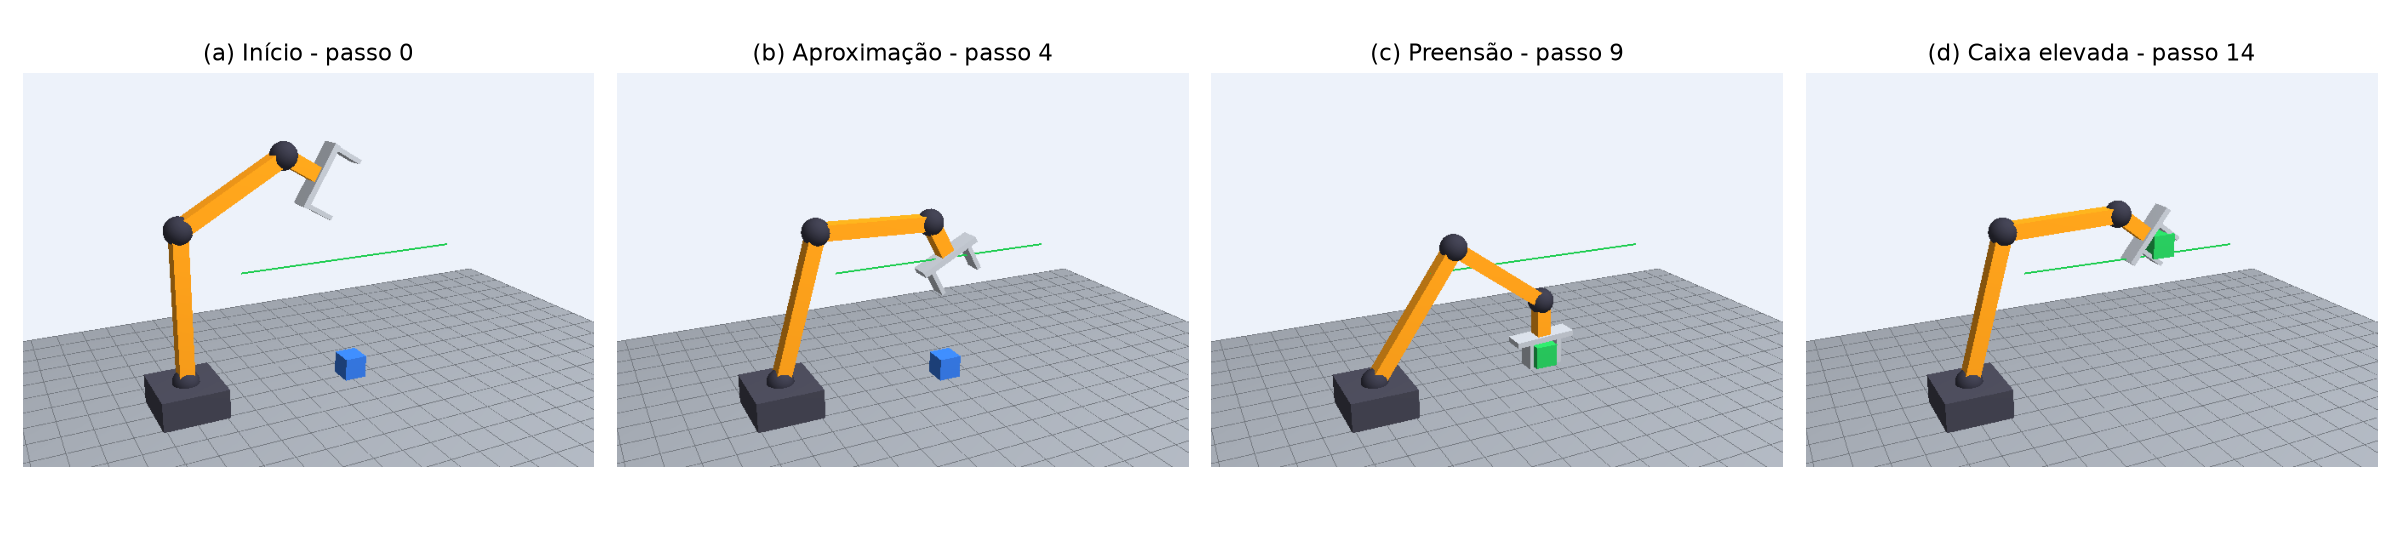
\includegraphics[width=\textwidth]{sequencia_sac.png}
    \caption{Episódio do SAC treinado, renderizado em OpenGL: (a) postura inicial; (b) aproximação; (c) preensão, com a caixa em verde indicando que está presa; (d) caixa elevada até a altura-alvo (linha verde).}
    \label{fig:sequencia}
\end{figure*}

\subsection{Discussão}

A diferença na eficiência de amostras está de acordo com o funcionamento dos algoritmos. O SAC armazena todas as transições no \textit{replay buffer} e realiza uma atualização a cada passo, reaproveitando cada experiência muitas vezes, inclusive as poucas em que o braço se aproximou ou agarrou a caixa. O PPO, por ser \textit{on-policy}, utiliza cada lote de 8.192 transições em apenas 10 épocas e depois o descarta, necessitando de mais interações para acumular o mesmo aprendizado. Em contrapartida, cada passo do PPO é computacionalmente mais barato e pode ser executado em vários ambientes em paralelo. O tempo de treinamento não foi comparado, pois os treinamentos foram executados simultaneamente na mesma máquina, disputando o processador, o que tornaria a medição pouco confiável.

O experimento com recompensa esparsa mostra que a recompensa em etapas acelerou o aprendizado, mas não foi indispensável nesta tarefa. Isso se deve, em grande parte, às simplificações do ambiente: o movimento ocorre em um plano, a caixa está sempre ao alcance do braço e a preensão é considerada bem-sucedida apenas pela distância e pelo fechamento da garra. Nessas condições, a exploração aleatória inicial do SAC foi suficiente para que alguns episódios de sucesso fossem encontrados e reaproveitados.

Algumas limitações devem ser consideradas. Os resultados se baseiam em uma única semente por configuração; como o desempenho de algoritmos de aprendizado por reforço varia entre execuções, a repetição com mais sementes é necessária para confirmar as diferenças observadas. A física simplificada, sem atrito e sem forças de contato, torna a tarefa mais fácil do que em um braço real, e a granularidade de 10.000 passos entre avaliações limita a precisão com que se pode identificar o momento do aprendizado.

\section{Conclusão}

Este trabalho apresentou um ambiente de simulação de um braço robótico com garra, renderizado em OpenGL, no qual o agente aprende sozinho, por aprendizado por reforço, a alcançar, agarrar e elevar uma caixa posicionada aleatoriamente. O braço possui três juntas rotacionais com limites angulares, sem rotação completa, e é controlado por ações contínuas. A renderização por modelagem hierárquica com a pilha de matrizes do OpenGL permitiu visualizar o comportamento aprendido, enquanto a separação entre simulação e renderização permitiu treinar os agentes sem interface gráfica.

Os dois algoritmos avaliados, PPO e SAC, aprenderam a tarefa e alcançaram 100\% de sucesso em 100 episódios de teste, concluindo-a em cerca de 15 passos. O SAC, por reaproveitar as experiências armazenadas, atingiu esse desempenho com aproximadamente 20.000 passos de treinamento, contra cerca de 110.000 do PPO, o que confirma a maior eficiência de amostras dos métodos \textit{off-policy} em problemas de controle contínuo. O experimento de controle mostrou ainda que a recompensa em etapas acelerou o aprendizado em cerca de três vezes em relação à recompensa esparsa.

Como trabalhos futuros, sugerem-se: repetir os experimentos com mais sementes, para dar validade estatística à comparação; adicionar uma junta de rotação da base, tornando o movimento tridimensional; adotar um motor de física com atrito e contato, como PyBullet ou MuJoCo; usar as imagens renderizadas pelo OpenGL como entrada do agente, no lugar das coordenadas; incluir várias caixas e a tarefa de empilhá-las; e, por fim, transferir a política aprendida para um braço físico.

\end{document}
